\documentclass{beamer}
\usepackage{kyradefaults}

% Custom UChicago theme color (Maroon)
\definecolor{uchicagored}{RGB}{128,0,0}
\setbeamercolor{footline}{fg=white,bg=uchicagored}

\usepackage[style=authoryear,backend=biber]{biblatex}
\addbibresource{references.bib}

\usepackage{tikz}
\usetikzlibrary{arrows.meta, positioning}
\usepackage{graphicx}
\usepackage{hyperref}
\usepackage{subcaption}
\usepackage{amsmath,amssymb}

% Theme setup
\usetheme{Madrid}
\usecolortheme[named=uchicagored]{structure}

% Footer
\setbeamertemplate{footline}{
  \leavevmode
  \begin{beamercolorbox}[wd=\paperwidth,ht=2.75ex,dp=1.25ex,left]{footline}
    \hspace{1em}
    \usebeamerfont{author in head/foot}Kyra Sadovi (UChicago Harris)
    \hfill
    \usebeamerfont{date in head/foot}\textit{All Aboard? New Rail Stations and Labor Markets}
    \hfill
    \usebeamerfont{date in head/foot}\insertshortdate
    \hspace{1em}
    \usebeamerfont{page number in head/foot}
    \insertframenumber{} / \inserttotalframenumber
  \end{beamercolorbox}
}

\setbeamertemplate{navigation symbols}{}

\title[New Rail Stations and Labor Markets]{All Aboard? Causal Evidence on\\Labor-Market Effects of New Rail Stations}
\author{Kyra Sadovi}
\institute{University of Chicago Harris School of Public Policy \\
\href{mailto:ksadovi@uchicago.edu}{ksadovi@uchicago.edu}}
\date{\today}

\useoutertheme{smoothbars}

% ============================================================
\begin{document}
% ============================================================

\begin{frame}[plain]
  \titlepage
\end{frame}

\begin{frame}[plain]{Outline}
  \tableofcontents
\end{frame}

% ============================================================
\section{Motivation}
% ============================================================

% ------ Slide 1 ------
\begin{frame}{The Policy Moment}
\small
\textbf{American cities are in a transit boom:}
\begin{itemize}
    \item New rail lines opening or under construction in LA, Seattle, DC, Boston, Miami, and beyond.
    \item Unprecedented urban congestion and surging demand to live in dense cities.
    \item % TODO: add a striking scale stat (e.g. FTA New Starts commitments, total VMT, etc.)
\end{itemize}

\medskip
\textbf{The political rationale for rail:} new stations expand economic opportunity for
nearby residents---better jobs, higher incomes, stronger communities.

\medskip
\textbf{But the case is contested:}
\begin{itemize}
    \item Critics: benefits flow to developers and landowners, not workers.
    \item Existing evidence focuses on land values and ridership, not individual labor outcomes
          \parencite{mcmillen_reaction_2004}.
    \item \textit{Does gaining access to a new rail station actually make nearby workers better off?}
\end{itemize}
\end{frame}

% ------ Slide 2 ------
\begin{frame}{The Obvious Mechanism---and Why It's Incomplete}
\small
\textbf{The standard story:} transit makes commuting more reliable.
\begin{itemize}
    \item Workers without cars can get to work more consistently $\Rightarrow$ lower job loss risk
          \parencite{sanchez_connection_1999, bastiaanssen_transport_employmentfx}.
    \item This is probably real---but it's a modest effect on its own.
\end{itemize}

\medskip
\textbf{The puzzle:} if transit only helps you keep your current job, why would we expect
to see income growth or job-to-job mobility? Yet the policy case for rail implicitly assumes
larger, more dynamic effects.

\medskip
\textbf{Something else must be going on.}

\medskip
A clue: in many cities, transit lines connect neighborhoods that would otherwise be
socially isolated from one another. The commute itself may be less important than
\emph{who else ends up in your network} as a result of gaining access.
\end{frame}

% ------ Slide 3 ------
\begin{frame}{Geographic Friction and Social Network Formation}
\small
\textbf{Your neighborhood determines your network.}

\medskip
\textcite{kim_spatial_2023}: social tie formation depends strongly on geographic distance.
\begin{itemize}
    \item Agents decide how often to visit others in a city, facing travel costs.
    \item Greater spatial dispersion $\Rightarrow$ fewer interactions $\Rightarrow$ lower social capital.
    \item Equilibrium interactions fall \emph{below} the social optimum because travel is costly.
\end{itemize}

\medskip
\textbf{Key result:} at equal cost, subsidizing interactions outperforms subsidizing
transportation---but subsidizing transportation does restore some of the social optimum.

\medskip
\textbf{What this implies for transit:} a new rail station doesn't just reduce commute time.
It lowers the effective cost of reaching a broader set of people---expanding the geographic
radius within which you form and maintain social ties.

\medskip
\textit{Transit is a partial subsidy to social interaction, operating through the
transportation cost channel.}
\end{frame}

% ------ Slide 4 ------
\begin{frame}{Why Networks Are Labor-Market Relevant}
\small
\textcite{patacchini_referral_fx}: using de-identified cellphone records from a Chinese city,
\begin{itemize}
    \item Information flow (call volume) correlates strongly with \textbf{worker flows} across
          geographic areas---a pattern that persists at all levels of aggregation.
    \item \textbf{Socioeconomic diversity} in social contacts is crucial: diversity in your
          information sources predicts job mobility more than raw contact volume.
    \item \textbf{Referred jobs are better}: higher wages, higher probability of going
          full-time, shorter commutes, higher probability of entering desirable occupations.
\end{itemize}

\medskip
\textbf{The chain:}
\[
\underbrace{\text{New station}}_{\text{lower travel cost}}
\;\Rightarrow\;
\underbrace{\text{broader social geography}}_{\text{\citeauthor{kim_spatial_2023}}}
\;\Rightarrow\;
\underbrace{\text{more diverse contacts}}_{\text{information flow}}
\;\Rightarrow\;
\underbrace{\text{better job matches}}_{\text{\citeauthor{patacchini_referral_fx}}}
\]

\medskip
\textbf{Implication for outcomes:} I should see job-to-job transitions and income growth,
not just employment retention---which is exactly what I measure.
\end{frame}

% ============================================================
\section{Research Question and Contribution}
% ============================================================

% ------ Slide 5 ------
\begin{frame}{Research Question and Outcomes}
\textbf{Goal:} Estimate the causal effect of gaining access to a new rail station on the
labor-market outcomes of nearby residents.

\bigskip
\textbf{Outcomes (from LODES):}
\begin{itemize}
    \item Worker flows: job retention and job-to-job transitions
    \item Income
\end{itemize}

\bigskip
\textbf{Three mechanisms I can speak to:}
\begin{enumerate}
    \item \textbf{Reliability:} more consistent commuting $\Rightarrow$ job retention.
    \item \textbf{Search radius:} wider job-search area $\Rightarrow$ better matches and higher wages.
    \item \textbf{Networks:} expanded social geography $\Rightarrow$ more referrals $\Rightarrow$
          faster and better transitions.
\end{enumerate}
\end{frame}

% ------ Slide 6 ------
\begin{frame}{Where This Fits in the Literature}
\small
\textbf{Market access and city structure:}
\begin{itemize}
    \item \textcite{tsivanidis_evaluating_2022}: TransMilenio (Bogotá BRT), structural model,
          firm location and spatial equilibrium. Focused on aggregate welfare, not individual
          worker trajectories.
    \item \textcite{baum-snow_does_2020}: national highways and city structure. City/region
          level, not individual outcomes, not quasi-experimental in the same sense.
    \item % TODO: add Donaldson/Hornbeck railroads + market access if relevant
\end{itemize}

\medskip
\textbf{Quasi-experimental transit work:}
\begin{itemize}
    \item \textcite{tyndall_airports}: airport rail lines $\uparrow$ local employment density.
          Place-level effects, IV using airport-station distance.
    \item \textcite{perez_urban_2022}: urban transit and spatial mismatch---closest to my setting
          but focuses on commuting patterns rather than worker-level transitions.
\end{itemize}

\medskip
\textbf{My contribution:}
\begin{itemize}
    \item \textbf{Substantive:} individual-level, residential-neighborhood channel for rail access.
    \item \textbf{Methodological:} recentered instrument (BH) adapted for the US multi-project
          context, combined with stacked DiD---novel in the transit literature.
\end{itemize}
\end{frame}

% ============================================================
\section{Identification Design}
% ============================================================

\subsection{Challenges}

% ------ Slide 7 ------
\begin{frame}{Three Identification Challenges}
\small
\begin{enumerate}
    \item \textbf{Anticipation effects}
    \begin{itemize}
        \item Long construction timelines mean behavior and prices adjust when a station is
              \emph{announced}, not when it opens.
        \item \textcite{mcmillen_reaction_2004}: house prices on the Chicago Orange Line
              capitalized benefits up to 6 years before completion.
        \item Standard event-study around realized opening date will be contaminated.
    \end{itemize}
    \medskip
    \item \textbf{Resident sorting}
    \begin{itemize}
        \item Workers with stronger labor-market attachment may select into transit-accessible
              neighborhoods.
        \item Cross-sectional patterns confound access with composition.
    \end{itemize}
    \medskip
    \item \textbf{Station location choice}
    \begin{itemize}
        \item Planners site stations in already-important locations: CBDs, dense residential
              areas, airports \parencite{tyndall_airports}.
        \item Naïve comparison of station areas vs.\ non-station areas picks up siting
              decisions, not access effects.
    \end{itemize}
\end{enumerate}
\end{frame}

\subsection{Delays as Timing Variation}

% ------ Slide 8 ------
\begin{frame}{Delays as a Timing Shock}
\small
\textbf{Key observation:} once a station is planned and approved, \emph{when} it opens
is shaped by construction complexity, permitting, and contractor issues---not by local
economic conditions.

\medskip
\textbf{My shock:} construction delays $D_s = R_s - P_s$ (realized minus planned opening date).

\medskip
\textbf{Project-time index:}
\begin{center}
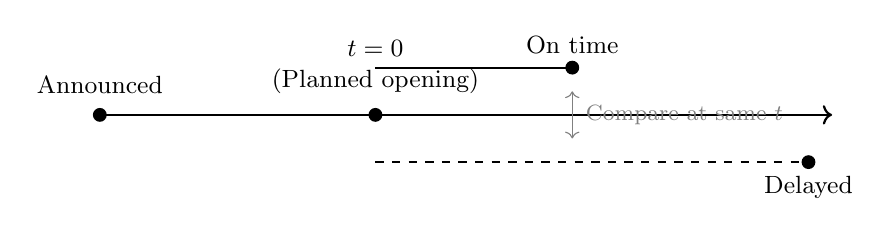
\begin{tikzpicture}[font=\small]
    \def\xA{0} \def\xB{3.5} \def\xC{6} \def\xD{9}
    % Axis
    \draw[->, thick] (\xA,0) -- (\xD+0.3,0);
    % Markers
    \foreach \x/\lab in {\xA/Announced, \xB/{$t=0$\\(Planned opening)}} {
        \fill (\x,0) circle (2.5pt);
        \node[above, align=center] at (\x, 0.15) {\lab};
    }
    % On-time branch
    \draw[thick] (\xB,0.6) -- (\xC,0.6);
    \fill (\xC,0.6) circle (2.5pt);
    \node[above] at (\xC,0.65) {On time};
    % Delayed branch
    \draw[thick, dashed] (\xB,-0.6) -- (\xD,-0.6);
    \fill (\xD,-0.6) circle (2.5pt);
    \node[below] at (\xD,-0.65) {Delayed};
    % Compare label
    \draw[<->, gray] (\xC, 0.3) -- (\xC,-0.3);
    \node[right, gray, font=\footnotesize] at (\xC+0.05,0) {Compare at same $t$};
\end{tikzpicture}
\end{center}

\medskip
\textbf{Design:} compare tracts near stations at the \emph{same} project-time $t$, one
open and one delayed. This addresses:
\begin{itemize}
    \item[$\checkmark$] \textbf{Siting:} both neighborhoods were already selected for a
          station---I only vary timing.
    \item[$\checkmark$] \textbf{Anticipation:} the project-time index is anchored to planned
          opening, so pre-period behavior shows up at $t<0$ for all projects equally.
\end{itemize}
\end{frame}

\subsection{Non-Random Exposure and BH Recentering}

% ------ Slide 9 ------
\begin{frame}{But Delays Alone Aren't Enough}
\small
\textbf{Problem:} even if delay \emph{timing} is quasi-random, \emph{exposure} to a new
station is not.

\medskip
Tracts near planned stations are systematically:
\begin{itemize}
    \item Denser and more central.
    \item Higher-income (on average).
    \item Already better-connected to the transit network.
\end{itemize}

\medskip
Using delays as an instrument for exposure will conflate the timing shock with these
pre-existing spatial differences---standard IV inherits the bias.

\medskip
\textbf{Solution:} \textcite{borusyak_nonrandom_2023} recentered instrument---subtract out
the \emph{expected} exposure implied by baseline geography, leaving only the surprise
component driven by realized delay timing.
\end{frame}

% ------ Slide 10 ------
\begin{frame}{Background: Why ``Random'' Shocks Aren't Enough}
\small
\textbf{A general problem in applied work:}

Many instruments are built from a formula combining an exogenous shock with
predetermined geography:
\[
    z_i = f(g;\, w_i)
\]
where $g$ is the shock (quasi-random) and $w_i$ is the unit's baseline characteristics (not random).

\medskip
\textbf{Classic example:} weather as an instrument for outdoor events.
\begin{itemize}
    \item Any given day's weather is random.
    \item But cities with better average climate will \emph{always} have more outdoor events,
          regardless of today's realization.
    \item The instrument picks up both the random-day component \emph{and} the
          systematic climate component.
\end{itemize}

\medskip
\textbf{In my setting:} tracts near dense, central stations gain more access under
\emph{any} delay realization---so the raw instrument is contaminated by baseline
geography even if delays themselves are quasi-random.

\medskip
\citeauthor{borusyak_nonrandom_2023}: this creates OVB even when shock timing is exogenous.
\end{frame}

% ------ Slide 11 ------
\begin{frame}{BH Solution: Recentering the Instrument}
\small
\textbf{Idea:} subtract out the part of exposure that is \emph{predictable} from
baseline geography. What remains is the surprise---driven purely by whether this particular
station happened to be delayed more or less than expected.

\medskip
\textbf{In practice:}
\begin{enumerate}
    \item Hold baseline geography $w$ fixed.
    \item Permute delay realizations $B$ times to simulate counterfactual schedules $g^{(b)}$.
    \item Compute expected exposure:
    \[
        \mu_{ct} = \frac{1}{B}\sum_{b=1}^{B} z_{ct}(g^{(b)};\, w)
    \]
    \item Recenter: $\tilde{z}_{ct} = z_{ct}(g;\,w) - \mu_{ct}$.
\end{enumerate}

\medskip
\textbf{Interpretation:} $\tilde{z}_{ct} > 0$ means this tract got access \emph{sooner than
its geography would have predicted}; $\tilde{z}_{ct} < 0$ means it was unexpectedly delayed.
Identification comes entirely from these surprises---\emph{not} from which neighborhoods
happen to be near stations.

\medskip
In 2SLS, $\tilde{z}_{ct}$ instruments for actual exposure while $\mu_{ct}$ is controlled for.
\parencite{borusyak_nonrandom_2023}
\end{frame}

% ------ Slide 12 ------
\begin{frame}{My Adaptation: What's Different from BH's China Application}
\small
\textcite{borusyak_nonrandom_2023} apply recentering to China's high-speed rail network:
permuting which HSR \emph{segments} open when, across an integrated national network.

\medskip
\textbf{Why that doesn't translate directly to the US:}
\begin{itemize}
    \item No single integrated US network---each project has its own institutional history,
          funding source, and construction management.
    \item Simulating a counterfactual US network structure is not credible when projects
          are locally approved, locally funded (via FTA New Starts), and locally managed.
    \item Their application also does not address anticipation effects.
\end{itemize}

\medskip
\textbf{My approach:}
\begin{itemize}
    \item Permute delays \emph{within cohorts} of similar stations (same line type
          $\times$ baseline centrality class) rather than simulating a network.
    \item The counterfactual question: among stations that faced similar
          institutional environments, which ones happened to open earlier vs.\ later?
    \item Project-time index handles anticipation explicitly.
\end{itemize}
\end{frame}

% ============================================================
\section{Data}
% ============================================================

% ------ Slide 13 ------
\begin{frame}{Building the Delay Dataset}
\small
\textbf{Transit Costs Project:} base list of major US rail projects, last $\sim$20 years.

\medskip
\textbf{EPA EIS Database:} for each project I record:
\begin{itemize}
    \item Announcement / DEIS finalization date
    \item Intended opening date $P_s$ (from the EIS)
    \item Realized opening date $R_s$
    \item Delay $D_s = R_s - P_s$
\end{itemize}

\medskip
\textbf{Result:} a hand-collected dataset of % TODO: insert N stations
US rail station openings with full project timelines.

\medskip
\textbf{Systems currently included:}
WMATA, MBTA, HART, LA Metro, Sound Transit, MTA (NYCT + LIRR),
VTA/BART, SF Muni, Miami-Dade Metrorail % TODO: verify completeness

\medskip
\textbf{Key data decision:} I use the \emph{first} projected opening date from the initial
DEIS---not later revisions---to avoid contaminating $P_s$ with information about delays
already underway.
\end{frame}

% ------ Slide 14 ------
\begin{frame}{Measuring Access and Outcomes}
\small
\begin{columns}[T]
\begin{column}{0.48\textwidth}
\textbf{Walking access (r5r):} \parencite{r5r}
\begin{itemize}
    \item Pedestrian routing on OpenStreetMap + GTFS.
    \item Pre-period network only (keeps exposure predetermined).
    \item Walking isochrones at 5, 10, 15 min from each tract centroid.
    \item Result: who is within walking distance of each station.
\end{itemize}
\medskip

\includegraphics[width=\textwidth]{3_output/2_figures/1_maps/1_station_geographies/WMATA.png}
\end{column}
\begin{column}{0.48\textwidth}
\textbf{Worker flows (LODES):}
\begin{itemize}
    \item Tract-level OD employment flows.
    \item Outcomes: worker inflows, outflows, job retention, income proxies.
\end{itemize}
\medskip

\includegraphics[width=\textwidth]{3_output/dmv_map.png}
\medskip
\textit{\footnotesize Currently using public tract-level data. Individual-level LODES
would allow person-level travel times and continuous CMA.}
\end{column}
\end{columns}
\end{frame}

% ============================================================
\section{Validation}
% ============================================================

% ------ Slide 15 ------
\begin{frame}{The Concern, Named Directly}
\small
\textbf{The most natural objection to my design:}

\begin{center}
\textit{``Delays are worse in economically struggling areas.\\
You're just comparing good neighborhoods to bad ones.''}
\end{center}

\medskip
If true: fiscal distress $\Rightarrow$ funding shortfalls $\Rightarrow$ delays;
fiscal distress also $\Rightarrow$ poor labor-market outcomes. Delays would be
correlated with pre-existing trends in exactly the outcomes I'm measuring.

\medskip
\textbf{This is the right concern, and I take it seriously.}

\medskip
Two tests:
\begin{enumerate}
    \item Do delays correlate with neighborhood income in the raw cross-section?
    \item Within a transit system (absorbing city-level institutional differences),
          do pre-period neighborhood characteristics predict delay length?
\end{enumerate}

\medskip
\textit{Next two slides.}
\end{frame}

% ------ Slide 16 ------
\begin{frame}{Test 1: Delay vs.\ Neighborhood Median Income}
\begin{center}
% TODO: insert figure path
% \includegraphics[width=0.85\textwidth]{PATH/TO/delay_vs_income_scatter.pdf}
\fbox{\parbox{0.85\textwidth}{\centering\vspace{3cm}
\textit{[Figure: Delay (days) vs.\ median household income by tract,}\\
\textit{colored by transit system, OLS line overlaid]}\\
\vspace{3cm}}}
\end{center}
\small
The regression line is essentially flat. System membership explains most of the
cross-sectional variation in delay---not neighborhood income.

\medskip
\textit{Note: Miami-Dade delay figure is being corrected.}
\end{frame}

% ------ Slide 17 ------
\begin{frame}{Test 2: Within-System Predictors of Delay}
\begin{center}
% TODO: insert figure path
% \includegraphics[width=0.85\textwidth]{PATH/TO/within_system_predictors.pdf}
\fbox{\parbox{0.85\textwidth}{\centering\vspace{3cm}
\textit{[Figure: Coefficient plot---effect of pre-period neighborhood characteristics}\\
\textit{on delay (days per SD), system FEs absorbed via demeaning]}\\
\vspace{3cm}}}
\end{center}
\small
After absorbing system fixed effects, \textbf{no labor-market characteristic predicts
delay length}. All 95\% CIs cross zero.

\medskip
Conditional on being in the same transit system, neighborhoods that waited longer
look the same as neighborhoods that opened on time.

\medskip
\textit{Wide CIs reflect limited station-level N---growing as I complete the dataset.}
\end{frame}

% ============================================================
\section{Empirical Specification}
% ============================================================

% ------ Slide 18 ------
\begin{frame}{Baseline 2SLS Specification}
\small
Let $x_{ct}$ be exposure (binary-band instrument or CMA) and $y_{ct}$ an outcome
(worker outflows, job-to-job transitions, income):

\medskip
\textbf{First stage:}
\[
x_{ct} = \pi\,\tilde{z}^{\text{bin}}_{ct} + \alpha\,\mu_{ct} + \Gamma' V_c + u_{ct}
\]

\textbf{Second stage:}
\[
y_{ct} = \beta\,\hat{x}_{ct} + \alpha\,\mu_{ct} + \Gamma' V_c + e_{ct}
\]

where $V_c$ includes tract and time fixed effects; $\mu_{ct}$ is controlled for
(not excluded) to isolate the surprise component \parencite{borusyak_nonrandom_2023}.

\medskip
\textbf{Exposure measure:}
\[
z^{\text{bin}}_{ct} = \sum_{s \in \mathcal{S}_c} O_{st}(g_t)\!\left[
\mathbf{1}\{d^{\text{walk}}_{cs} \le 5\}
+ \tfrac{2}{3}\mathbf{1}\{5 < d^{\text{walk}}_{cs} \le 10\}
+ \tfrac{1}{3}\mathbf{1}\{10 < d^{\text{walk}}_{cs} \le 15\}
\right]
\]
Weights encode decreasing influence with walk time; I test robustness to single cutoffs
and to a continuous CMA measure \parencite{eaton_technology_2002, donaldson_railroads_2016}.
\end{frame}

% ------ Slide 19 ------
\begin{frame}{My Contribution: Stacked DiD + Recentered Instrument}
\small
2SLS estimates a static average but hides: (i) dynamic effects over event time,
(ii) which cohorts drive the estimate.

\medskip
\textbf{Framework} \parencite{wing_stacked_2024}:
\begin{itemize}
    \item Define adoption time $A_c$ = realized station opening for tract $c$'s nearest station.
    \item Event time $e = t - A_c$; window $e \in [\kappa_{\text{pre}}, \kappa_{\text{post}}]$.
    \item For each adoption year $a$: sub-experiment with treated tracts ($A_c = a$)
          vs.\ not-yet-treated controls.
    \item Stack sub-experiments; apply WFH corrective weights to recover trimmed ATT.
\end{itemize}

\medskip
\textbf{Two options for $\tilde{z}_{ct}$:}
\begin{enumerate}
    \item Treat $\tilde{z}_{ct}$ as the treatment directly---event-time coefficients
          capture causal effects of an exogenous access increase.
    \item Stacked IV: instrument $x_{ct}$ (CMA or band exposure) with $\tilde{z}_{ct}$
          within the stacked panel.
\end{enumerate}

\medskip
\textbf{Why this is new:} combining BH recentering with stacked DiD has not been done
in the transit literature and provides a clean, dynamic ATT with a well-defined
comparison group.
\end{frame}

% ============================================================
\section{Open Questions}
% ============================================================

% ------ Slide 20 ------
\begin{frame}{What I'm Wrestling With}
\small
\textbf{1. City-level confounding without city fixed effects}
\begin{itemize}
    \item The by-system delay variation is large (Hawaii and Massachusetts vs.\ Florida).
          This isn't random---it reflects institutional, regulatory, and political differences.
    \item I don't have enough station-level observations for city or system fixed effects
          to fully absorb these differences.
    \item Current approach: within-system validation (Slide 17) + permute only within cohorts.
    \item \textit{Open question: is within-system validation convincing on its own, or do I
          need to restrict to multi-project systems?}
\end{itemize}

\medskip
\textbf{2. Limited station-level N}
\begin{itemize}
    \item Wide CIs in the validation---identification rests on a relatively small number
          of delay realizations.
    \item Miami data correction will help; so will extending to additional systems.
    \item \textit{Open question: what's the minimum credible N for this design?}
\end{itemize}
\end{frame}

% ------ Slide 21 ------
\begin{frame}{Next Steps and What I Want From You}
\small
\textbf{Immediate:}
\begin{itemize}
    \item Fix Miami-Dade delay figure and re-run validation.
    \item Redo the by-system delay disaggregation (currently by state).
    \item Complete the delay dataset for remaining systems.
    % TODO: add other immediate data steps
\end{itemize}

\medskip
\textbf{Medium term:}
\begin{itemize}
    \item Apply for individual-level LODES access (unlocks person-level travel times
          and continuous CMA).
    \item Run first-stage regressions once dataset is complete.
    \item Implement the stacked DiD + recentered instrument specification.
\end{itemize}

\medskip
\textbf{I want feedback on:}
\begin{enumerate}
    \item \textbf{City FEs:} how do you handle this kind of cross-city confounding with
          limited observations?
    \item \textbf{Validation:} is the within-system null result (Slide 17) sufficient, or
          do I need additional evidence that delays are exogenous?
    \item \textbf{Mechanisms:} any suggestions for separating the reliability,
          search-radius, and network channels empirically?
\end{enumerate}
\end{frame}

% References
\begin{frame}[noframenumbering,plain,allowframebreaks]{References}
    \printbibliography[heading=none]
\end{frame}

\end{document}